%METADATA about GPU, purpose and general difference from CPU
\section{Graphics Processing Units}
Graphic Processing Units (GPUs) were initially used to accelerate memory-intensive work for rendering graphics.
They consist of a higher amount of cores, these cores while each less powerfull than the cores used in a CPU, are so plentiful that with enough work, more data can be processed in parallel.
These cores sacrifice the architectural components that enables the CPU run single instruction streams in exchange for more computing power, such as increasing the number of \textbf{Arithmetic Logic Units (ALUs)} \myref{image:GPUCPUimage} shows a basic idea of the difference between the GPU and CPU. %http://pdsgroup.hpclab.ceid.upatras.gr/files/CUDA-Parallel-Computing-on-GPUs.pdf
\begin{figure}[h!]
\centering
 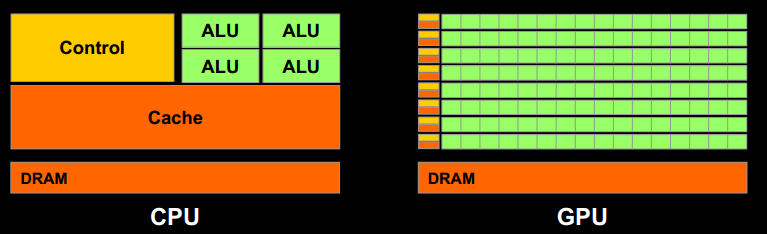
\includegraphics[width=1\textwidth]{figures/GPUCPUimage.png} % trim=4.85cm 15cm 0.85cm 1cm
\caption{A basic representation of the Transistor allocation on a GPU compared to a CPU}\label{image:GPUCPUimage} %ftp://download.nvidia.com/developer/cuda/seminar/TDCI_Arch.pdf
\vspace{-25pt}
\end{figure}

This concept of using many cores to process a high number of threads gives GPUs a high throughput, and is therefore a main principal of GPUs.
In recent years GPUs have been used for more than just graphical purposes, such as GPU-accelerated computing, the use of both GPU and CPU to accelerate scientific and analytical applications.
%http://www.nvidia.com/object/what-is-gpu-computing.html



%GPU Architecture
\subsection{GPU architecture}
For the purpose of this section it is worth noting that depending on the GPU manufacturer and the series of the GPU, the exact architecture may vary.
This section will therefore describe the architecture in a conceptual manor, and not go into specifics. 
Also note that the main difference between earlier and later models of the same manufacturer, is primarily size of memory, not the architectural concepts themselves.
The GPU architecture chosen as the basis for the following section is NVIDIA. 
They are the market share leader, discounting integrated graphics solutions. 
	%Kernels
	%SingleInstructionMultipleData (SIMD)
The GPU consists of compute units (\textbf{Streaming Multiprocessors (SMs)}) which each consists of processing elements (\textbf{Streaming Processors (SPs)}), registers, execution cores for integer and floating point operations as well as several caches; shared memory, texture memory and constant memory cache.
%http://www.cudahandbook.com/uploads/Chapter_8._Streaming_Multiprocessors.pdf
For GPU-accelerated computing the GPU acts as a co-processor for data which can be calculated in parallel.
The GPU is controlled by the CPU.
The CPU calls the GPU driver and starts a data transfer with the GPU or a \textbf{kernel} launch on the GPU.
A kernel is a function executed on the GPU. %, this is explained further on \myref{sec:opencl}.
A kernel specifies the number of threads and data it requires.
%http://www.cs.virginia.edu/~skadron/Papers/thesis_prateeksha.pdf
%GPU Memory Hierachy
\subsection{Memory Hierachy}
	%Register (per-SM, allocated to threads as specified - fastest and most plentiful)	
	%Local memory (SM holds local variables that cannot be computed at compile time) texture cache
	%Global (GPU) Visible to all threads of a kernel, resides in DRAM 
	%Constant memory (GPU) Each SM contains a small latency optimized cache for purpose of reading this memory DRAM
	%Shared memory (per-SM, shared amongst threads of a block) Seperate adress space
	%Host memory (CPU)

%http://www.cudahandbook.com/uploads/Chapter_8._Streaming_Multiprocessors.pdf
\begin{figure}[h!]
\centering
 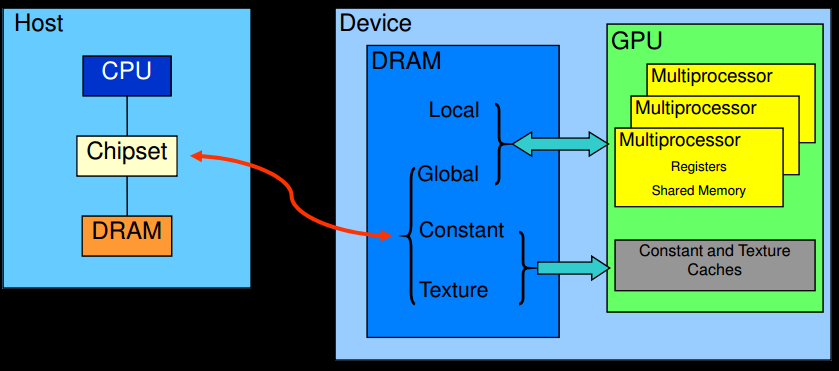
\includegraphics[width=1\textwidth]{figures/GPUMemoryClear.png} % trim=4.85cm 15cm 0.85cm 1cm
\caption{A basic representation of GPU memory hierarchy}\label{image:GPUMemory} 
\end{figure}
The GPU memory is comprised of the following different memory components, how it communicates is shown on \todo{OpenCLGPUMemoryModel}. 
Memory management of the GPU is also explicit, this means that the data must first be moved from the host, to global memory, then to local memory where the SMs can start to use it. 
Once they are done the result must be sent back the same way.
The memory architecture is designed with regard to performance by reducing memory traffic.
Although the hierarchy and its components were originally designed to improve performance for graphical applications, it can also be used efficiently in some GPU computing applications, how the memory is used is further explained in \todo{Advanced OpenCL}. %http://cuda-programming.blogspot.dk/2013/02/texture-memory-in-cuda-what-is-texture.html

\textbf{Registers:}

For any given SM, thousands of registers are contained, this is the most plentiful type of memory used in the SM. 
Once a kernel is launched, registers are allocated to threads as per the kernels requirements.
This also means that the registers are shared across the SM, but only to the allocated thread.
When allocated the registers are no longer available to the entire SM, once the thread is done and they can be reallocated.
The registers can each contain either integers and floating-points.

\textbf{Local Memory:}

Local memory is used for spilling registers as well as holding local variables.
Each SM has its own allocated local memory available which is available to the entire SM, unlike registers it is not controlled by the kernel being executed.

\textbf{Global and Constant Memory:}

The SMs can read and write to global memory, this is significantly slower than using local memory. %http://www.it.uu.se/edu/course/homepage/avdark/ht10/slides/09-GPU-and-OpenCL-4.pdf
Constant memory is read only for the SM however each SM contains a small optimized cache for the purpose of reading from this memory such that less reading is required. 
Both of these memory types are located on the DRAM and not in the SM.

\textbf{Shared Memory:}

Shared memory, as mentioned earlier, is part of the SM.
It is a very fast on-chip memory that threads can use for data interchange within thread blocks.
Although it is fast, being an on-chip per-SM resource, using it can affect the number of blocks and threads can used for computations.

\textbf{Texture Memory:}

Texture memory is shared amongst a number of SMs, like constant memory this is read-only for the SM and is cached in its own texture cache on the SM.

%Streaming Multiprocessors
\begin{wrapfigure}{r}{0.25\textwidth}
 \vspace{-50pt}
 \begin{center}
  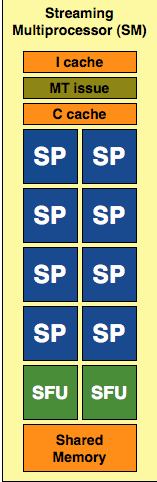
\includegraphics[width=0.23\textwidth]{figures/SM.png}
 \end{center}
 \caption{A basic representation of a SM.}\label{image:SM} 
 \vspace{-35pt}
\end{wrapfigure}
\subsection{Streaming Multiprocessors}
On the GPU the work is divided by the hardware.
When a kernel is launched, the hardware dynamically assigns work groups to SMs, doing so while balancing the load across the GPU.
For each work group, a number of work items exists, these are the threads which execute the kernels.
Work items running on a SM can communicate through local memory, all the different work groups can communicate through global memory. %https://www.khronos.org/assets/uploads/developers/library/2009-hotchips/NVIDIA_OpenCL-for-NVIDIA-GPUs.pdf
A collection of a given number of SMs is referred to as a \textbf{Thread Processing Cluster (TPC)}, this TPC shares a controller as well as a texture cache.
All SMs consists of a number of ALUs, \textbf{multiply-add (MAD)} and special function units for doing computations, multi-threaded instruction fetch and issue unit, instruction cache, read-only constant cache and a shared memory cache.
\myref{image:SM} shows an example of this, note that the ALUs and MAD corresponds to the SPs.
The SM schedules and executes threads in groups called warps.
A warp waits until all its threads have finished executing, before the next instruction is fetched. 


%http://www.cs.virginia.edu/~skadron/Papers/thesis_prateeksha.pdf
\subsection{Conclusion} %This needs serious rework - but not now!

The architectural difference of the GPU from the CPU, are intended to maximise the throughput for problems that can handle a higher latency.
The lack of control and cache memory for the processing units used in the GPU, also greatly reduces its capabilities of handling complex issues that requires a concurrent approach.
Since the GPU does not have interupts an instruction in a given thread will run until it is complete and no thread will start without all the available resources.
Thus some problems will be ill suited for the GPU but any problems that can be divided into smaller blocks of data, and designated to run on different threads, will benefit substantially from the increased computing power the GPU provides.
The scheduling of said blocks are controlled by the hardware and no explicit management is required.
In conclusion due to the magnitude of threads available in a GPU, its memory hierarchy for said threads and the ability of the hardwares to manage those threads, any problem with data parallel workloads will be executed significantly faster than on any equivalent CPU.

%First Draft
%The result of this architecture is increased parallel computing power through the sacrifice of sequential computing power.
%The GPU sacrifices the cache memory of the CPU, in exchange for more computing power.
%This results in a very high throughput, work done in an amount of time, given that there is enough work.
%It also results in higher latency, the time from which an instruction is initiated untill the effects have taken place.
%Is is the direct opposite of a CPU.
%In a CPU low latency is preferred, the latency is hidden through its ability to do work concurrently the low latency is achieved by the caches, something which the GPU sacrificed.
%Although with low latency, also follows low throughput, which is why the GPU is more optimized for heavy computational work that can be done in parallel.
%The structure of SMs, and the work distribution of the GPU, is what enables it to use the SIMD model.
%The SM follows only one set of instructions but on multiple threads of data, the threads are managed and scheduled by the hardware itself.
%In conlusion, the GPU architecture allows us to efficiently compute any workload which can be done using parallel computing, and can tolerate the higher latency.

%GPU Results Parallel work/Multiprocessor programming
	%Latency/Throuhput optimizations and the result